\documentclass[tikz,border=5pt]{standalone}
\usepackage{amsmath,amssymb}
\begin{document}
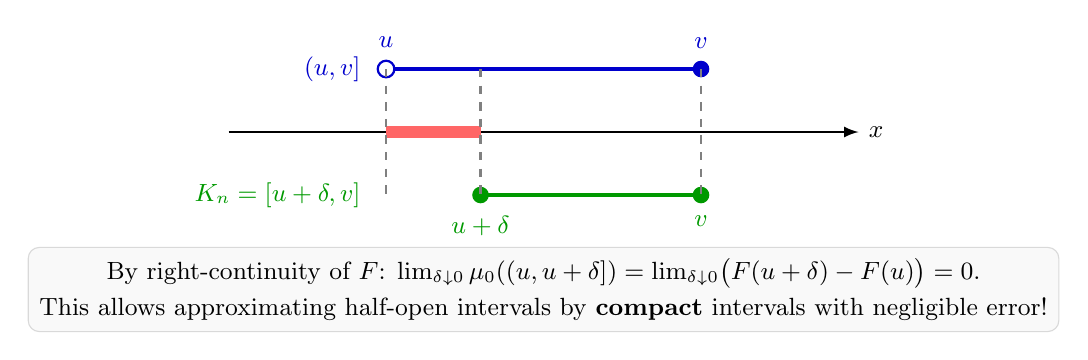
\begin{tikzpicture}[>=latex, font=\small]
  % Real axis
  \draw[->, thick] (-1, 0) -- (7, 0) node[right] {$x$};

  % Original half-open interval (u, v]
  \draw[very thick, blue!80!black] (1, 0.8) -- (5, 0.8);
  \draw[thick, blue!80!black, fill=white] (1, 0.8) circle (3pt) node[above=4pt] {$u$};
  \fill[blue!80!black] (5, 0.8) circle (3pt) node[above=4pt] {$v$};
  \node[blue!80!black, left] at (0.8, 0.8) {$(u, v]$};

  % Shrunken compact interval K_n = [u + delta, v]
  \draw[very thick, green!60!black] (2.2, -0.8) -- (5, -0.8);
  \fill[green!60!black] (2.2, -0.8) circle (3pt) node[below=4pt] {$u + \delta$};
  \fill[green!60!black] (5, -0.8) circle (3pt) node[below=4pt] {$v$};
  \node[green!60!black, left] at (0.8, -0.8) {$K_n = [u+\delta, v]$};

  % Difference slice
  \draw[line width=4pt, red!60!white] (1, 0) -- (2.2, 0);
  \draw[thick, dashed, gray] (1, 0.8) -- (1, -0.8);
  \draw[thick, dashed, gray] (2.2, 0.8) -- (2.2, -0.8);
  \draw[thick, dashed, gray] (5, 0.8) -- (5, -0.8);

  \node[align=center, fill=gray!5, draw=gray!30, rounded corners, inner sep=4pt] at (3.0, -2.0)
    {By right-continuity of $F$: $\lim_{\delta \downarrow 0} \mu_0((u, u+\delta]) = \lim_{\delta \downarrow 0} \bigl(F(u+\delta) - F(u)\bigr) = 0$.\\[2pt]
     This allows approximating half-open intervals by \textbf{compact} intervals with negligible error!};
\end{tikzpicture}
\end{document}
